\newpage
\section{Theoretische Grundlagen (11-11,5)}
\label{TheoretischeGrundlagen}
In diesem Kapitel werden die statistischen Grundlagen für die Modellierung vorgestellt. Zuerst wird die deskriptive Analyse definiert und beschrieben. Danach wird die lineare Regression beschrieben. Der \autoref{einfuehrungInDieRegression} umfasst einfache und multiple lineare Regression. Nach der linearen Regression werden die Einschränkungen der Regression aufgelistet. Es gibt Voraussetzungen, um ein lineares Modell zu trainieren. Es wird diskutiert, wie der Umgang mit den Einschränkungen ist. Eine gängige Methode für die lineare Regression ist die Methode der kleinsten Quadrate. Deshalb wird darauffolgend die Methode der kleinsten Quadrate mathematisch erklärt. Anschließend werden Werte wie Bestimmtheitsmaß vorgestellt, die Gültigkeit eines Modells messen. Nachfolgend wird die Methode der kleinsten absoluten Abweichungen als robustere Schätzung vorgestellt, und zum Schluss werden die Huber-Loss-Funktion, die Methode der kleinsten Quadrate und die Methode der absoluten Abweichungen integriert.
\subsection{Deskriptive Analyse}
\label{deskriptiveanalyse}
Die deskriptive Analyse stellt einen wichtigen Schritt im Prozess der Datenwissenschaft im Marketing dar, da sie ein umfassendes Verständnis von historischen Daten vermittelt. Sie ermöglicht es den Marketern, wesentliche Muster, Trends und Beziehungen in den Daten zusammenzufassen, zu visualisieren und zu interpretieren. Somit bildet die deskriptive Analyse Grundlagen für fortgeschrittenere Analysen wie prädiktive und präskriptive Analysen. Die deskriptive Analyse ist essenziell, um Kundenverhalten und -präferenzen zu verstehen, Markttrends und Konkurrenzdynamik zu identifizieren, Marketingeffekte zu evaluieren und Entscheidungsfindung im datengesteuerten Marketing zu unterstützen \cite{brown2024mastering}. \\\\
Deskriptive, prädikative und präskriptive Analysen haben verschiedene Verwendungszwecke und Methoden. Die deskriptive Analyse benutzt die Statistik, Datenaggregation und Visualisierung, um das vergangene Verhalten zusammenzufassen und zu verstehen. Sie wird verwendet in Markttrendanalysen, Kundensegmentierung und Analysen der Verkaufsleistung mithilfe der Reports, Dashboards und Charts. Basierend auf historischen Daten wird die prädiktive Analyse verwendet, um den zukünftigen Verlauf vorherzusagen. Dabei entstehen Vorhersagen und Wahrscheinlichkeitswerte auf Grundlagen von Regressionen, maschinellem Lernen und Zeitreihenanalysen. Sie wird verwendet für die Vorhersage der Kundenabwanderung und Absatzprognose. Zum Schluss wird die präskriptive Analyse verwendet, um Maßnahmen für die Zukunft zu empfehlen. Dabei werden Optimierung, Simulation und Entscheidungsbaum angewandt, um Empfehlungen und Entscheidungsmodelle zu erzeugen. Diese Analyse wird verwendet, um die Preisoptimierung, Kampagnenausrichtung und das Bestandsmanagement zu unterstützen. Die deskriptive Analyse hat ein breiteres Analysenspektrum und ergänzt andere Analysen in effektiven Marketingstrategien\cite[S. 51 ff]{brown2024mastering}. 


\subsection{Einführung in die lineare Regression}
\label{einfuehrungInDieRegression}
Die lineare Regression ist eines der am häufigsten eingesetzten Werkzeuge in der Datenanalyse und im Rahmen der fundamentalen Analysemethoden deckt sie den Bereich Prognose ab \cite{frick2021data}.  \\\\
Regressionsanalysen modellieren Zusammenhänge zwischen unabhängigen und abhängigen Variablen. Die unabhängigen Variablen werden als Eingabe in das Modell eingegeben und die abhängige Variable soll prognostiziert werden. Die lineare Regression setzt voraus, dass ein linearer Zusammenhang zwischen den Variablen besteht. Die lineare Regression kann als Formel ausgedrückt werden in der \autoref{eq:simpleregression} \cite{frick2021data}. 
\begin{equation}
Y = \beta_0 + \beta_1 X + \epsilon \tag{3.1}
\label{eq:simpleregression}
\end{equation}
Sei \(X\) eine unabhängige Variable und Y eine abhängige Variable. Durch diese Gleichung wird eine Regressionsgerade gezogen. Die Regressionsanalyse schätzt den Steigungsparameter $\beta_1$ und den Achsenabschnitt $\beta_0$. Die in das Diagramm eingetragenen Punkte heißen Beobachtungen. Das Modell kann genutzt werden, den \(y'_i\)-Wert für die jeweiligen \(x_i\)-Werte vorherzusagen und mit dem tatsächlichen \(y_i\) zu vergleichen. Da in der Regel kein vollständiger linearer Zusammenhang zwischen den Variablen vorliegt, besteht ein Unterschied zwischen manchen Beobachtungen und der Regressionsgerade. Der vertikale Abstand zwischen einer Beobachtung und der Regressionsgerade wird Residuum genannt. Das Residuum stellt eine Schätzung für den Fehlerterm $\epsilon$ (\anf{Epsilon}) dar und wird in der Gleichung berücksichtigt \cite{frick2021data}.  \\\\
Wenn mehrere unabhängige Variablen in das Modell eingegeben werden, ist das ein \ac{MLR}. Die Formel wird erweitert für mehr \(x\)-Werte. In der \autoref{eq:multilinear} wird die \ac{MLR} beschrieben \cite{frick2021data}. 
\begin{equation}
Y = \beta_0 + \beta_1 X_{1} + \beta_2 X_{2} + \dots + \beta_p X_{p} + \varepsilon, \tag{3.2}
\label{eq:multilinear}
\end{equation}
\(p\) bezeichnet dabei die Anzahl der unabhängigen Variablen. Das \ac{MLR}-Modell ähnelt dem der linearen Regression und unterstellt ebenfalls einen linearen Zusammenhang \cite{frick2021data}. Im \ac{MMM} können die abhängigen Variablen Preis, digitale Ausgaben, Zeitungs- und Magazinkosten, TV-Kosten etc. sein und die Ausgabe-Variable kann Nachfrage, Marktanteil und Gewinn sein \cite{akinkunmi2018data}.
\\\\
Um die optimalen Schätzwerte in einer klassischen linearen Regression zu ermitteln, wird meistens die Methode der kleinsten Quadrate (engl. \ac{OLS}) oder eine Maximum Likelihood-Schätzung (engl. \ac{MLE}) verwendet. In beiden Fällen wird die Summe der kleinsten Abweichungsquadrate (engl. \ac{RSS}), um für die Daten optimale Modellwerte zu liefern \cite[S. 246]{frick2021data}. 
\subsection{Einschränkungen der Regression}
\label{einschränkungenderregression}
Bei dem Einsatz einer einfachen linearen oder einer multiplen linearen Regression können folgende Probleme auftauchen \cite{james2013introduction}: 
\begin{itemize}
    \item \textbf{Nichtlinearität der Beziehungen zwischen der Antwortvariablen und den Prädiktoren:} Das Modell nimmt an, dass ein linearer Zusammenhang besteht. Wenn das nicht der Fall ist, führt dies zu Fehlschätzungen. 
    \item \textbf{Korrelation der Fehlerterme:} Das Modell setzt voraus, dass die Fehlerterme voneinander unabhängig sind. Wenn sie miteinander korreliert sind, kann das zu verzerrten Ergebnissen führen.
    \item \textbf{Nicht-konstante Varianz der Fehlerterme:} Die Varianz der Fehlerterme sollte konstant bleiben. Wenn sie variiert, kann die Unsicherheit in den Schätzungen nicht korrekt abgeschätzt werden.
    \item \textbf{Ausreißer:} Einzelne Punkte, die sehr weit entfernt von den meisten Datenpunkten liegen, können das Modell stark verzerren.
    \item \textbf{Datenpunkte mit großer Hebelwirkung:} Einige Punkte mit extremen \(x\)-Werten üben großen Einfluss auf das Modell aus und können es unverhältnismäßig beeinflussen.
    \item \textbf{Multikollinearität:} Wenn zwei Merkmale stark miteinander korreliert sind, kann das Modell die individuellen Effekte dieser Variablen nicht eindeutig abschätzen.
\end{itemize}
Diese Probleme können nach der Modellerstellung mithilfe grafischer Darstellungen überprüft werden. Solange Auffälligkeiten bestehen, sollten die Daten oder das Modell nicht in der gedachten Form verwendet werden. Allerdings können die Daten, die die Voraussetzungen nicht erfüllen, durch eine Datentransformation angepasst werden. Beispielsweise kann das lineare Modell bei der Wertentwicklung eines Sparkontos nicht eingesetzt werden, da durch den Zinseszinseffekt ein exponentieller Zusammenhang besteht. Die Logarithmierung des Kontowerts erzeugt einen nahezu linearen Zusammenhang. Nach der Datentransformation ist darauf zu achten, dass die Datenbasis verändert wird und die Interpretation entsprechend angepasst werden muss. In dem Fall ist der Koeffizient der unabhängigen Variablen nicht mehr die Steigerung in der Einheit des Kontowertes, sondern eine prozentuale Steigerung. Je nach Transformationsart ist die Interpretation mit Sorgfalt zu überprüfen \cite{akinkunmi2018data}. \\\\
Eine Methode, um die Kollinearität aufzudecken, ist die Untersuchung der Korrelationsmatrix der Prädiktoren. Wenn ein hoher absoluter Wert in der Matrix auftritt, weist dies auf ein Paar hoch korrelierter Variablen hin und somit auf ein Kollinearitätsproblem in den Daten. Es ist möglich, dass Kollinearität zwischen mehreren Variablen besteht, ohne dass eine hohe Korrelation zwischen allen Variablen auftritt. Diese Situation wird als Multikollinearität bezeichnet.\\\\
Zusammenfassend ist die \ac{MLR} eine grundlegende und wichtige Methode der Datenanalyse und erfordert Aufmerksamkeit, weil die Prognose außerhalb der 
bekannten Daten mit Unsicherheit verbunden ist \cite{akinkunmi2018data}. 

\subsection{Methode der kleinsten Quadrate}
\label{methodederkleinstenquadrate}
Die Methode der kleinsten Quadrate, \ac{OLS}, ist die am häufigsten verwendete Methode, um das lineare Modell zu trainieren (s. \autoref{eq:RSS}). 
\begin{equation}
RSS(\beta) = \sum_{i=1}^{N} (y_i - x_i^T \beta)^2 
\label{eq:RSS}
\end{equation}
In diesem Ansatz wird der Koeffizient $\beta$ so gewählt, dass die Summe der quadrierten Residuen (engl. \ac{RSS}) minimiert wird \cite{hastie2009elements}. Die \autoref{eq:RSS} stellt die Summe der quadrierten Abweichungen zwischen den tatsächlichen und den geschätzten Ausgabewerten dar. 
\begin{equation}
f(X) = \beta_0 + \sum_{j=1}^{p} X_j \beta_j 
\label{eq:linearOLS}
\end{equation}
Die \autoref{eq:linearOLS} stellt die lineare Regression dar. Ein Eingabevektor \( X^T = (X_1, X_2, \ldots, X_p) \) wird als Trainingsdaten gegeben und in die \autoref{eq:linearOLS} eingesetzt. Dieses Modell geht davon aus, dass die Regressionsfunktion E(X|Y) linear ist, oder dass das lineare Modell eine vernünftige Schätzung liefert. Dabei sind die $\beta_j$ die unbekannten Parameter bzw. Koeffizienten, und die \( X_j \) können verschiedene Datentypen repräsentieren. Die \( X_j \) können quantitative Eingaben oder transformierte quantitative Eingaben sein. Beispielsweise können transformierte quantitative Eingaben logarithmierte, quadrierte oder Wurzel gezogene Werte sein. Sie können aus einer erweiterten Basis stammen, wie \( X_2 = X_1^2, \quad X_3 = X_1^3,\quad \ldots \) Ebenso können sie kodierte, qualitative Eingaben darstellen, z.B. durch Umwandlung kategorialer Werte in numerische Werte wie 1 und 0. Schließlich können sie Werte darstellen, bei denen eine Interaktion zwischen den Variablen besteht, wie \( X_3 = X_1 \cdot X_2 \) \cite{hastie2009elements}.\\\\
Normalerweise wird mit Trainingsdaten wie \( ( (x_1, y_1) \cdots (x_N, y_N) ) \) gearbeitet, um den Parameter $\beta$ zu schätzen. Jeder \( x_i = (x_{i1}, x_{i2}, \ldots, x_{ip})^T \) ist ein Vektor der Merkmalsmessungen für den \(i\) -ten Fall. In der Methode der kleinsten Quadrate werden Koeffizienten \( \beta \equiv (\beta_0, \beta_1, \ldots, \beta_p)^T \) gewählt, um die \ac{RSS} zu minimieren \cite{hastie2009elements}. Die \ac{RSS} ist gegeben durch:
\begin{equation}
RSS(\beta) = \sum_{i=1}^{N} (y_i - f(x_i))^2 
= \sum_{i=1}^{N} \left( y_i - \beta_0 - \sum_{j=1}^{p} x_{ij} \beta_j \right)^2
\label{eq:rsshoch2}
\end{equation}
Aus statistischer Sicht ist dieses Kriterium valide, wenn die Beobachtungen \( (x_i, y_i) \) eine unabhängige, zufällige Stichprobe aus der Population darstellen. Auch wenn die \(x_i\)-Werte nicht zufällig sind, bleibt es immer noch gültig, wenn die \(y_i\)-Werte unter der Bedingung der gegebenen Eingaben \(x_i\) bedingt unabhängig sind \cite{hastie2009elements}.  \\\\
Die \autoref{eq:rsshoch2} stellt jedoch nicht die Gültigkeit des Modells sicher, sondern liefert lediglich die beste lineare Anpassung an die Daten. Die Methode der kleinsten Quadrate ist intuitiv befriedigend, ohne dabei die Entstehung der Daten zu berücksichtigen. Das Kriterium misst den durchschnittlichen Anpassungsfehler. \\\\
Dabei sei X eine \( N \times (p + 1) \) Matrix, wo jede Zeile ein Eingabe-Vektor ist. Jeder Vektor beginnt mit einer 1, um die $\beta_0$ Koeffizienten zu ermöglichen. Sei \(y\) ein \(N\)-Vektor der Ausgaben für die Trainingsdaten. Dann kann die \ac{RSS} als Formel so ausgedrückt werden: 
\begin{equation}
RSS(\beta) = (y - X\beta)^T (y - X\beta).
\label{eq:RSSmatrix}
\end{equation}
Das ist eine quadratische Funktion mit \(p + 1\) Parametern. Diese wird nach $\beta$ abgeleitet:
\begin{equation}
\begin{aligned}
\frac{\partial RSS}{\partial \beta} &= -2 X^T (y - X\beta) \\
\frac{\partial^2 RSS}{\partial \beta \partial \beta^T} &= 2 X^T X.
\end{aligned}
\label{eq:RSSableitung}
\end{equation}
Unter der Annahme, dass \( X \) vollen Rang \( p \) besitzt \cite{huber1981robust}, sind die Spalten von \( X \) linear unabhängig. Das bedeutet, dass keine Spalte von \( X \) als Vielfaches oder lineare Kombination der anderen Spalten dargestellt werden kann. Sei dabei die Matrix \( X^T X \) auch positiv definit, was sicherstellt, dass die Lösung für \( \beta \) eindeutig ist \cite{hastie2009elements}. Dann wird die erste Ableitung gleich 0 gesetzt und nach $\beta$ eindeutig aufgelöst: 
\begin{equation}
\begin{aligned}
0 &= -2 X^T (y - X\beta) \quad  \\
0 &= X^T (y - X\beta) \quad  \\
  &= X^T y - X^T X \beta \\
X^T X \beta &= X^T y \\
\beta &= (X^T X)^{-1} X^T y \\
\hat{\beta} &= (X^T X)^{-1} X^T y \quad \text{($\hat{\beta}$ geschätzter Parameter)}
\end{aligned}
\label{XTXderived}
\end{equation}
Wenn die Spalten von \( X \) linear abhängig sind, besitzt \( X \) keinen vollen Rang \cite{hastie2009elements}. In diesem Fall liegt Kollinearität vor \cite{Maronna2019Robust}. Dies geschieht, wenn zwei Eingaben perfekt miteinander korrelieren. In diesem Fall ist \(X^TX\) singular und der Koeffizient der kleinsten Quadrate $\hat{\beta}$ ist nicht eindeutig definiert \cite{hastie2009elements}. Nicht eindeutig bedeutet, dass es Vektoren \(\beta_1 \neq \beta_2 \text{ gibt, sodass } X\beta_1 = X\beta_2\). Dies impliziert, dass die Funktion unendlich viele Lösungen für $\hat{\beta}$ hat \cite{Maronna2019Robust}. In der Praxis tritt der Fall unvollständiger Rangbedingungen am häufigsten auf, wenn eine oder mehrere qualitative Eingaben redundant kodiert sind. In der Regel lässt sich die nicht-eindeutige Darstellung beheben, indem die Kodierung der qualitativen Daten angepasst oder redundante Spalten in X entfernt werden \cite{hastie2009elements}. \\\\
Die Matrix \( H = X (X^T X)^{-1} X^T \) in der \autoref{hutmatrix} wird als \anf{Hutmatrix} genannt. Da sie einen \anf{Hut} auf \(y\) setzt \cite{huber1981robust}. 

\begin{equation}
\hat{y} = X \hat{\beta} = X(X^T X)^{-1} X^T y \quad 
\label{hutmatrix}
\end{equation}
Es wird klar, dass \(H\) eine symmetrische \( n \times n \) Projektionsmatrix ist. Das heißt, \( HH = H \): 
\begin{equation}
\begin{aligned}
H H &= \left( X (X^T X)^{-1} X^T \right) \left( X (X^T X)^{-1} X^T \right) \\
&= X (X^T X)^{-1} (X^T X) (X^T X)^{-1} X^T \\
&= X (X^T X)^{-1} X^T \\
&= H
\end{aligned}
\label{eq:idempotent}
\end{equation}
Und dass sie \(p\) Eigenwerte gleich 1 und \( n - p \) Eigenwerte gleich 0 hat \cite{huber1981robust}. Ihre diagonalen Elemente \(h_i\) befriedigen:
\begin{equation}
0 < h_i < 1  \label{eq:hi_condition}
\end{equation}
Und die Spur von H ist p: 
\begin{equation}
\text{tr}(H) = p \label{eq:trace_H}
\end{equation}
\(tr(H)\) ist die Summe der diagonalen Elemente von H. Die diagonalen Elemente enthalten wichtige Informationen. Ein großer \(h_i\)-Wert weist auf eine Warnung hin und bedeutet, dass die \(i\)-te Beobachtung einen entscheidenden, aber nicht überprüfbaren Einfluss haben könnte. Ein h < 0,2 scheint unproblematisch zu sein, ein h-Wert zwischen 0,2 und 0,5 ist riskant. Wenn es in der Kontrolle ist, sollte ein h < 0,5 vermieden werden \cite{huber1981robust}. \\\\
Aus geometrischer Sicht hat \(\hat{y}\) den kürzesten Abstand zu \(y\) aufgrund der Orthogonalität. Die Spaltenvektoren von X werden mit \(x_0, x_1, \ldots, x_p\) bezeichnet. Dabei ist \(x_0\) der Vektor mit konstantem Wert 1. Diese Vektoren bilden einen Unterraum von $\mathbb{R}^N$ auf und werden in die Formel \( RSS(\beta) = \|y - X\beta\|^2 \) eingesetzt, um das Ergebnis zu minimieren. Nach der Minimierung entsteht ein Parameter $\hat{\beta}$, sodass der Residuum-Vektor \(y-\hat{y}\) orthogonal zu diesem Unterraum steht. Daher stellt \(\hat{y}\) die orthogonale Projektion von \(y\) dar. Die \anf{Hut}-Matrix berechnet diese orthogonale Projektion, daher wird sie auch Projektionsmatrix genannt \cite{hastie2009elements}. 
\subsection{Anpassungsgüte und die Varianzanalyse}
\label{AnpassungsgüteUndDieVarianzanalyse}
Um die Anpassungsgüte eines Modells zu beschreiben, wird das Bestimmtheitsmaß verwendet. Sei dabei \ac{SST} die gesamte Streuung der abhängigen Variable \( y \) um den Mittelwert \( \bar{y} \) und das \(e\) das Residuum. Weiterhin sei die \ac{SSM} die durch das Modell erklärte Streuung und \ac{RSS} die Streuung der Residuen. Dann wird das Bestimmtheitsmaß beschrieben durch: 
\begin{equation}
\frac{RSS}{SST} = \frac{\beta^{T}X^{T}M_{y}\beta}{y^{T}M_{y}y} = 1 - \frac{e^{T}e}{y^{T}M_{y}y}.
\label{R2kurz}
\end{equation}
Das Bestimmtheitsmaß hat die Notation  \( R^2 \) und liegt zwischen 0 und 1. Es misst den Anteil der Gesamtvariation in \(y\), der durch die Variation der Prädiktoren erklärt wird. Das Bestimmtheitsmaß beträgt 0, wenn die Regression eine horizontale Gerade ist. Das bedeutet, dass alle Prädiktoren $\beta_j$s (außer $\beta_0$) gleich 0 sind. In diesem Fall ist der vorhergesagte $y$ Wert immer $\bar{y}$ und die Abweichung des $x$ von dem Mittelwert wird nicht in die Vorhersage für $y$ berücksichtigt. So hat x keine Aussagekraft. Der andere extreme Fall \(R^2\)=1 tritt auf, wenn alle \(x\) und \(y\) Werte auf einer Gerade liegen, sodass alle Residuen 0 sind. Wenn alle Werte von $y_i$ auf einer orthogonalen Linie liegen, hat $R^2$ keine Bedeutung und es kann nicht berechnet werden.  \\\\ 
Regressionen werden oft für die Vorhersage verwendet. 
In diesem Fall wird untersucht, wie gut das Regressionsmodell die Veränderungen der abhängigen Variablen vorhersagt. Eine äquivalente Methode zur Berechnung von $R^2$ kann dargestellt durch: 
\begin{equation}
R^2 = \frac{\left[\sum_{i}(y_i - \bar{y})(\hat{y}_i - \hat{y})\right]^2}{\left[\sum_{i}(y_i - \bar{y})^2\right]\left[\sum_{i}(\hat{y}_i - \hat{y})^2\right]}
\label{R2Formel}
\end{equation}
$R^2$ ist die quadrierte Korrelation zwischen den Beobachtungen und den vom Modell erzeugten Vorhersagen \cite{greene2003econometric}.\\\\
Auch die Hypothese zu einem spezifischen Koeffizienten kann überprüft werden.  
\begin{equation}
t_k = \frac{(b_k - \beta_k)/\sqrt{\sigma^2 S^{kk}}}{\sqrt{[(n-K)s^2/\sigma^2]/(n-K)}} = \frac{b_k - \beta_k}{\sqrt{s^2 S^{kk}}}
\label{eq:tk_formula}
\end{equation}
In der \autoref{eq:tk_formula} wird eine t-Verteilung mit (n - K) Freiheitsgraden beschrieben. \(n\) ist die Anzahl der Stichproben, K ist die Anzahl der Koeffizienten. \(b_k\) ist der berechnete Koeffizient und $S^{kk}$ steht für das \(k\)-te Element in \((X^TX)^{-1}\). \(t_k\) kann verwendet werden, um die Hypothese zu überprüfen oder um ein Konfidenzintervall für die individuellen Elemente des $\beta$s zu formen.  \cite{greene2003econometric}.\\\\
Ein üblicher Test besteht darin, die Signifikanz zu überprüfen, ob $\beta$ von null abweicht. Die geeignete Teststatistik wird durch \autoref{eq:t_formula} dargestellt. 
\begin{equation}
t = \frac{b_k}{s_{b_k}}
\label{eq:t_formula}
\end{equation}
Der Wert \(t\) ist in den meisten Computerprogrammen als Teil der Standardausgaben zu finden. Diese Statistik wird in der Regel als \(t\)-Verhältnis (\(t-ratio\)) für den Schätzer \(b_k\) bezeichnet. Wenn \( \left|\frac{b_k}{s_{b_k}}\right| > t_{\alpha/2} \), wird die Hypothese abgelehnt. Dabei ist \( t_{\alpha/2} \) der 100 (1 - \(\alpha\)/2)-Prozent-kritische Wert der \(t\)-Verteilung mit (n - K) Freiheitsgraden, und der Koeffizient wird als statistisch signifikant anerkannt. Wenn die Tabelle der kritischen Werte nicht sofort verfügbar ist und es sich um große Stichproben handelt, wird der Wert 1,96 als Richtwert für ein Signifikanzniveau von 5 \% verwendet. Das \(t\)-Verhältnis ist in den meisten Computerprogrammen ein zentraler Bestandteil der Regressionsanalyse. Dabei ist es für den Test der Hypothese, dass ein Koeffizient null ist. \\\\
Der \autoref{einschränkungenderregression} beschreibt das Problem der Kollinearität und das Erkennen der Kollinearität durch die Korrelationsmatrix. Statt des Untersuchens der Korrelationsmatrix kann die Multikollinearität durch den \ac{VIF} aufgedeckt werden. Der \ac{VIF} misst den Einfluss der Kollinearität auf die Varianz von $\hat{\beta_j}$. Er wird berechnet, indem die Varianz von $\hat{\beta_j}$ im vollständigen Modell durch die Varianz von $\hat{\beta_j}$ in einem Modell ohne andere Prädiktoren dividiert wird. Der kleinstmögliche Wert des \ac{VIF} ist 1, was ein vollständiges Fehlen von Kollinearität bedeutet. In der Praxis tritt ein kleiner Anteil an Kollinearität zwischen den Prädiktoren auf. Als Faustregel gilt ein \ac{VIF}-Wert über 5. Spätestens ab einem Wert von 10 weist dieser auf eine problematische Kollinearität hin \cite{james2013introduction}. \\\\
\begin{equation}
VIF(\hat{\beta}_j) = \frac{1}{1 - R^2_{X_j|X_{-j}}}
\label{vif}
\end{equation}
wobei \( R^2_{X_j|X_{-j}} \) das \( R^2 \) aus einer Regression von \( X_j \) auf alle anderen Prädiktoren ist. Wenn \( R^2_{X_j|X_{-j}} \) nahe bei eins liegt, ist Kollinearität vorhanden, und der VIF wird groß sein \cite{james2013introduction}.\\\\
\subsection{Methode der kleinsten absoluten Abweichungen}
\label{MethodeDerKleinstenAbsolutenAbweichungen}
Die Methode der kleinsten Quadrate (\ac{OLS}, s. \nameref{methodederkleinstenquadrate}) kann durch Ausreißer wesentlich verzerrt werden. Insbesondere in der Praxis der Mikro- und Finanzökonomie, da dort dickschwänzige Störverteilungen auftreten, die die Wahrscheinlichkeit solcher Verzerrungen erhöhen. Diese Herausforderungen haben zur Entwicklung sogenannter \anf{robuster} Schätzer geführt, die weniger von ausreißenden Beobachtungen beeinflusst werden. Die Methode der kleinsten absoluten Abweichungen, \ac{LAD}, ist einer der robusten Schätzer.\\\\
Die \ac{OLS} weist großen Abweichungen ein hohes Gewicht zu, was dazu führt, dass kleine oder mittlere Datensätze aufgrund einiger unüblicher Daten anfällig sind. Die Methode der kleinsten absoluten Abweichungen (\ac{LAD}) wurde als eine Alternative vorgeschlagen, die das Problem behebt. 
\begin{equation}
\label{eq:minimization}
\min_{\mathbf{b}_0} \sum_{i=1}^{n} \left| y_i - \mathbf{x}_i^T \mathbf{b}_0 \right|
\end{equation}
In der \autoref{eq:minimization} wird der Schätzer \(b_0\) so bestimmt, dass die Summe der Beträge der Abweichungen zwischen \(x_i^Tb_0\) und \(y_i\) minimal ist. Die Abweichungen werden für jede Beobachtung berechnet, und die Summe über alle Beobachtungen wird berechnet. \\\\
Die Methode der absoluten Abweichungen entstand vor der Entstehung der Methode der kleinsten Quadrate, die vor mehr als 200 Jahren entstand. In der Finanzökonomie wird der \ac{LAD}-Schätzer weniger verwendet und er wurde bei der Einführung von \ac{OLS} verdrängt. Er wurde verdrängt, weil \ac{OLS} viel einfacher zu berechnen ist. Außerdem sind die statistischen Eigenschaften von \ac{OLS} in der modernen Forschung besser etabliert als die \ac{LAD}. Und in der Regel sind die Stichproben groß genug, dass der Vorteil des \ac{LAD} bei kleinen Stichproben nicht mehr relevant ist. \\\\
Der \ac{LAD}-Schätzer ist ein Spezialfall der Quantilregression, der ausgedrückt wird durch: 
\begin{equation}
\label{eq:probability}
\text{Prob}[y_i \leq x_i^T\beta] = q.
\end{equation}
Der \ac{LAD}-Schätzer schätzt die Medianregression. Dabei ist die Lösung die Quantilregression, wenn q = 0,5. Das heißt, \(\beta\) wird so gewählt, dass 50 \% der \(y_i\)-Werte der Stichproben kleiner oder gleich \(x_i^T \beta\) sind. 
\subsection{Huber-Loss-Funktion}
\label{huberregression}
Im Jahr 1964 veröffentlichte Huber das Paper \anf{Robust Estimation of A Location Parameter}, in dem er einen neuen Ansatz zur robusten Schätzung vorstellte. Das Papier thematisiert die Schätzung eines Lageparameters in einer kontaminierten Normalverteilung. Huber versucht, mehr Robustheit zu erreichen, indem er eine andere Funktion der Fehler minimiert als die Summe ihrer Quadrate. Damit argumentiert Huber, dass die tatsächliche Verteilung der Daten von der angenommenen Verteilung abweichen könnte und somit ein falsches arithmetisches Mittel liefert. Eine leichte Abweichung könnte die Varianz sprengen. Es gab schon Substitute für das arithmetische Mittel wie den getrimmten Mittelwert, Windsorizing etc., aber eine allgemeine Theorie der robusten Statistik fehlte noch. Somit bildete Huber die Grundlagen der robusten Statistik in diesem Papier \cite{huberpapier}. \\\\
Die Huber-Loss-Funktion ist eine Mischung aus quadratischem Verlust für relativ kleine Fehler und absolutem Verlust für relativ große Fehler, während das Grad der Mischung von einem Tuning-Parameter gesteuert wird \cite{indirekthuber}. 
\\\\
Traditionelle Schätzmethoden summieren die Abweichungen der Datenpunkte und gewichten sie oft quadratisch. Dies führt dazu, dass Ausreißer besonders stark in das Ergebnis einfließen. Dadurch können die Schätzungen ungenau werden, wenn die Daten stark von der erwarteten Verteilung abweichen.    \\\\
Die Huber-Loss-Funktion ist definiert als:
\begin{equation}
\rho(t) = 
\begin{cases} 
  \frac{1}{2} |t|^2 & \text{for } |t| < k, \\ 
  k |t| - \frac{1}{2} k^2 & \text{for } |t| \geq k 
\end{cases}
\label{eq:huber}
\end{equation}
Die Huber-Loss-Funktion ist für kleine \(x\)-Werte quadratisch und für große \(x\)-Werte linear. Der Parameter \(k\) steuert die Mischung zwischen linearer und quadratischer Penalisierung. Die Methode der kleinsten Quadrate und die Methode der kleinsten absoluten Abweichungen (\ac{LAD}) können als zwei Extremfälle der Huber-Loss-Funktion betrachtet werden. Abweichend vom traditionellen Huber-Schätzer konvergiert der \(k\) gegen 0, um Verzerrungen bei der Schätzung in der mittleren Regressionsfunktion zu reduzieren, wenn die bedingte Verteilung nicht symmetrisch ist. Allerdings darf \(k\) nicht zu schnell sinken, um die Robustheit zu erhalten \cite{indirekthuber}. \\\\
Die \autoref{fig:verlustfunktionvergleich} vergleicht die drei Verlustfunktionen, \ac{OLS}, \ac{LAD} und die Huber-Loss-Funktion. Die \(x\)-Achse stellt die Abweichung zwischen dem Schätzer und der Beobachtung dar und die \(y\)-Achse stellt die Gewichtung dar. Die quadratische Verlustfunktion legt bei endlichen Stichproben deutlich mehr auf Beobachtungen mit großen absoluten Residuen \(|y-f(x)|\) während des Anpassungsprozesses. Daher ist sie weniger robust und ihre Leistung verschlechtert sich wesentlich bei stark fehlerhaft gemessenen \(y\)-Werten (Ausreißer). Andere robuste Methoden, wie die absolute Verlustfunktion, schneiden bei Ausreißern besser ab \cite{hastie2009elements}. 
\begin{figure}[H]
    \centering
    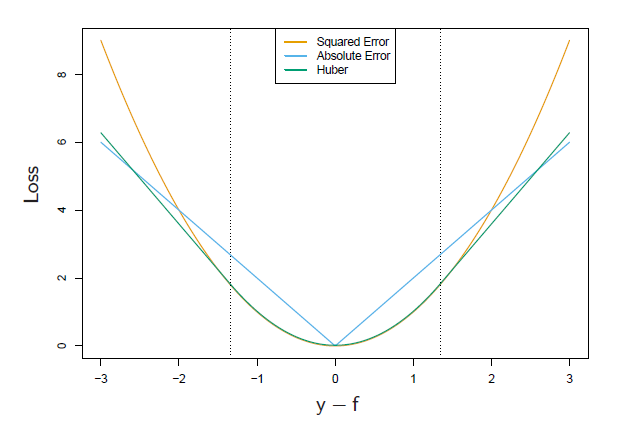
\includegraphics[width=1\linewidth]{images/3losses.png}
    \caption{Vergleich der drei Verlustfunktionen: \ac{OLS}, \ac{LAD} und Huber-Loss-Funktion \cite{hastie2009elements}}
    \label{fig:verlustfunktionvergleich}
\end{figure} 
\noindent
Im Bereich der Regression besteht eine Beziehung zwischen der quadratischen Verlustfunktion \((y - f(x))^2\) und der absoluten Funktion \(|y - f(x)|\). Für die quadratische Verlustfunktion ist die optimale Vorhersage der durchschnittliche Wert von \(Y\), wenn \(x\) bekannt ist. Für die absolute Verlustfunktion ist die optimale Vorhersage der Wert, bei dem die Hälfte der möglichen Werte von \(Y\) kleiner und die andere Hälfte größer als dieser Wert ist \cite{hastie2009elements}. Die Huber-Loss-Funktion wechselt zwischen diesen beiden Ansätzen, je nach Größe des Residuums.